\chapter{The Complex Number System}
%% I HAVE ADDED EXAMPLES OF EACH OF THE THEOREMSTYLES AND HOW TO USE THEM.
\noindent Complex number's day-to-day application is not as direct as that of real numbers, their imaginary component makes complex numbers important as they make it possible to work very precisely in specific areas of science and physics. This is the case with measuring electromagnetic fields, which consist of electrical and magnetic components and require pairs of real numbers to describe them. These pairs can be seen as a complex number, hence their importance.
\section{The Real Number System}
The number system as we know it today is a result of gradual development as indicated in the following list.
\begin{enumerate}
    \item Natural Numbers: $1,2,3,4, \ldots \ldots$.
    \item Negative integers and zero: $0,-1,-2,-3,-4, \ldots \ldots$
    \item Rational Numbers:
$\displaystyle \left\{x \mid x\right.$ is in the form $\displaystyle \left.\frac{a}{b}, b \neq 0\right\}$
\item Irrational Numbers:
$\displaystyle \left\{x \mid x\right.$ is not in the form $\displaystyle \left.\frac{a}{b}, b \neq 0\right\}$
\item Real Number:
\{Rational Number Set \} $\cup$ \{Irrational Number \}
\end{enumerate}
\noindent Real numbers can be represented by points on a line called the real axis, as indicated in Figure \ref{fig1}. The point
corresponding to zero is called the origin.
\begin{figure}[ht!]
    \centering
    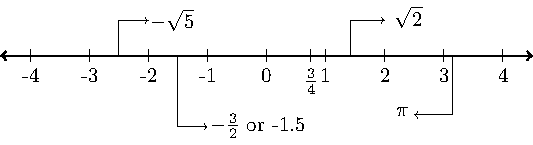
\includegraphics{FIG_MAT215/FIG1.pdf}
    \caption{}
    \label{fig1}
\end{figure}
\section{The Complex Number System}
There is no real number $x$ that satisfies the polynomial equation $x^2+1=0$. To permit solutions of this and similar equations, the set of complex numbers is introduced.
\begin{defn}
    A complex number takes the form $z=a+i b$ where $a$ and $b$ are real, and $i$ is an imaginary number that satisfies $i^2=-1$. We call $a$ and $b$ the real part and the imaginary part of $z$, respectively, and we write
$$
a=\operatorname{Re}(z) \quad \text { and } \quad b=\operatorname{Im}(z) .
$$
\end{defn}
\noindent The real numbers are precisely those complex numbers with zero imaginary parts. 
\begin{defn}
    A complex number with zero real part is said to be purely imaginary.
\end{defn}
\begin{theorem}
    Two complex numbers $a+b i$ and $c+d i$ in Cartesian coordinate system are equal if and only if $a=c$ and $b=d$.
\end{theorem}
\noindent  We can consider real numbers as a subset of the set of complex numbers with $b=0$. Accordingly the complex numbers $0+0 i$ and $-3+0 i$ represent the real numbers 0 and -3 , respectively. If $a=0$, the complex number $0+b i$ or $b i$ is called a pure imaginary number.
\begin{defn}[Complex Conjugate]
    The complex conjugate, or briefly conjugate, of a complex number $a+b i$ is $a-b i$. The complex conjugate of a complex number $z$ is often indicated by $\bar{z}$ or $z^*$.
    \begin{center}
    $ z=a+i b \hspace{0.5cm} \longrightarrow \hspace{0.5cm} \text{(Complex Number)}$\par 
$\bar{z}=a-i b  \hspace{0.5cm} \longrightarrow \hspace{0.5cm}$ (Complex conjugate of $z$ )
\end{center}
\end{defn}
\section{Fundamental Operations of Complex Numbers}
In performing operations with complex numbers, we can proceed as in the algebra of real numbers, replacing $i^2$ by -1 or $i^3$ by $-i$ or $i^4$ by 1 when it occurs and so on.
\begin{corollary}
    \textbf{Addition}
$$
(a+b i)+(c+d i)=a+b i+c+d i=(a+c)+(b+d) i
$$
\end{corollary}
\begin{corollary}
    \textbf{Subtraction}
$$
(a+b i)-(c+d i)=a+b i-c-d i=(a-c)+(b-d) i
$$
\end{corollary}
\begin{corollary}
    \textbf{Multiplication}
$$
(a+b i)(c+d i)=a c+a d i+b c i+b d i^2=(a c-b d)+(a d+b c) i
$$
\end{corollary}
\begin{corollary}
    \textbf{Division}\par 
\noindent If $c \neq 0$ and $d \neq 0$, then
$$
\begin{aligned}
\frac{a+b i}{c+d i} & =\frac{a+b i}{c+d i} \cdot \frac{c-d i}{c-d i}=\frac{a c-a d i+b c i-b d i^2}{c^2-d^2 i^2} \\
& =\frac{a c+b d+(b c-a d) i}{c^2+d^2}=\frac{a c+b d}{c^2+d^2}+\frac{b c-a d}{c^2+d^2} i
\end{aligned}
$$
\end{corollary}
\begin{defn}[Absolute Value]
    The absolute value or modulus of a complex number $a+b i$ is defined as $|a+b i|=\sqrt{a^2+b^2}$.
\end{defn}
\begin{ex}
    $|-4+2 i|=\sqrt{(-4)^2+(2)^2}=\sqrt{20}=2 \sqrt{5}$
\end{ex}
\begin{corollary}
    If $z_1, z_2, z_3, \ldots, z_m$ are complex numbers, the following properties hold.\par 
\noindent (1) $\displaystyle \left|z_1 z_2\right|=\left|z_1\right|\left|z_2\right| \quad$ or $\displaystyle\quad\left|z_1 z_2 \cdots z_m\right|=\left|z_1\right|\left|z_2\right| \cdots\left|z_m\right|$\par 
\noindent (2) $\displaystyle\left|\frac{z_1}{z_2}\right|=\frac{|z_1|}{|z_2|}\quad$ if $\displaystyle\quad z_2 \neq 0$\par 
\noindent (3) $\displaystyle\left|z_1+z_2\right| \leq\left|z_1\right|+\left|z_2\right| \quad$ or $\displaystyle\quad\left|z_1+z_2+\cdots+z_m\right| \leq\left|z_1\right|+\left|z_2\right|+\cdots+\left|z_m\right|$\par 
\noindent (4) $\displaystyle\left|z_1 \pm z_2\right| \geq\left|z_1\right|-\left|z_2\right|$
\end{corollary}
\section{Graphical Representation of Complex Numbers}
Okay, to visualize complex numbers in the complex plane we have several ways: 
\begin{enumerate}
    \item Rectangular form
    \item Polar form
    \item Exponential form
\end{enumerate}
Throughout our presentation, the set of all complex numbers is denoted by $\mathbb{C}$. The complex numbers can be visualized as the usual Euclidean plane by the following simple identification: the complex number $z=x+i y \in \mathbb{C}$ is identified with the point $(x, y) \in \mathbb{R}^2$. For example, 0 corresponds to the origin and $i$ corresponds to $(0,1)$. Naturally, the $x$ and $y$ axis of $\mathbb{R}^2$ are called the real axis and imaginary axis, because they correspond to the real and purely imaginary numbers, respectively.
\begin{figure}[ht!]
    \centering
    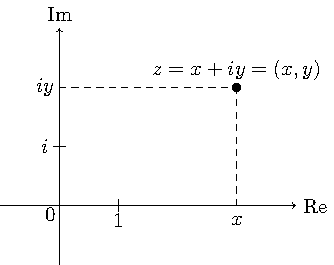
\includegraphics{FIG_MAT215/FiG2.pdf}
    \caption{ The Complex Plane}
    \label{fig2}
\end{figure}
\FloatBarrier
\begin{defn}
    The distance between two complex numbers, $z_1=x_1+i y_1$ and $z_2=x_2+i y_2$ is,
$$
\left|z_1-z_2\right|=\sqrt{\left(x_1-x_2\right)^2+\left(y_1-y_2\right)^2}
$$
\end{defn}

\begin{ex}
     The distance between $z_1=4-5 i$ and $z_2=-i$ is
$$
\begin{aligned}
\left|z_1-z_2\right| & =\sqrt{(4-0)^2+(-5+1)^2} \\
& =\sqrt{16+16}=\sqrt{32}=4 \sqrt{2}
\end{aligned}
$$
\end{ex}
\section{Polar Form of Complex Number}
Any non-zero complex number $z$ can be written in polar form
$$
z=r e^{i \theta},
$$
where $r>0$; also $\theta \in \mathbb{R}$ is called the argument of $z$ (defined uniquely up to a multiple of $2 \pi$ ) and is often denoted by $\arg z$, and
$$
\displaystyle e^{i \theta}=\cos \theta+i \sin \theta .
$$

\noindent Since $\left|e^{i \theta}\right|=1$ we observe that $r=|z|$, and $\theta$ is simply the angle (with positive counterclockwise orientation) between the positive real axis and the half-line starting at the origin and passing through $z$.
\begin{figure}[ht!]
    \centering
    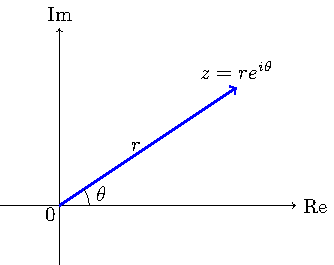
\includegraphics{FIG_MAT215/FIG3.pdf}
    \caption{The polar form of a complex number}
    \label{fig3}
\end{figure}
\FloatBarrier
\begin{theorem}
    Two complex numbers $z_1=r_1e^{i\theta_1}$ and $z_2=r_2e^{i\theta_2}$ in the polar coordinate will be equal if $$r_1=r_2 \quad \quad \theta_1=\theta_2+2k\pi \quad \quad \text{ where } k=0,\pm 1, \pm 2, \pm 3, ..........$$ 
\end{theorem}
\begin{defn}
    In order to make the argument of $z$ a well-defined number, it is sometimes restricted to the interval $(-\pi,\pi]$. This special choice is called the principal value or the main branch of the argument and is written as 
$Arg(z)$.
\end{defn}
\section{Finding Principal Argument}
Consider a complex number $z=x+i y$ or $(x, y)$ on the complex plane. Define, $\displaystyle\alpha=\tan ^{-1}\left(\left|\frac{y}{x}\right|\right)$
\begin{figure}[ht!]
    \centering
    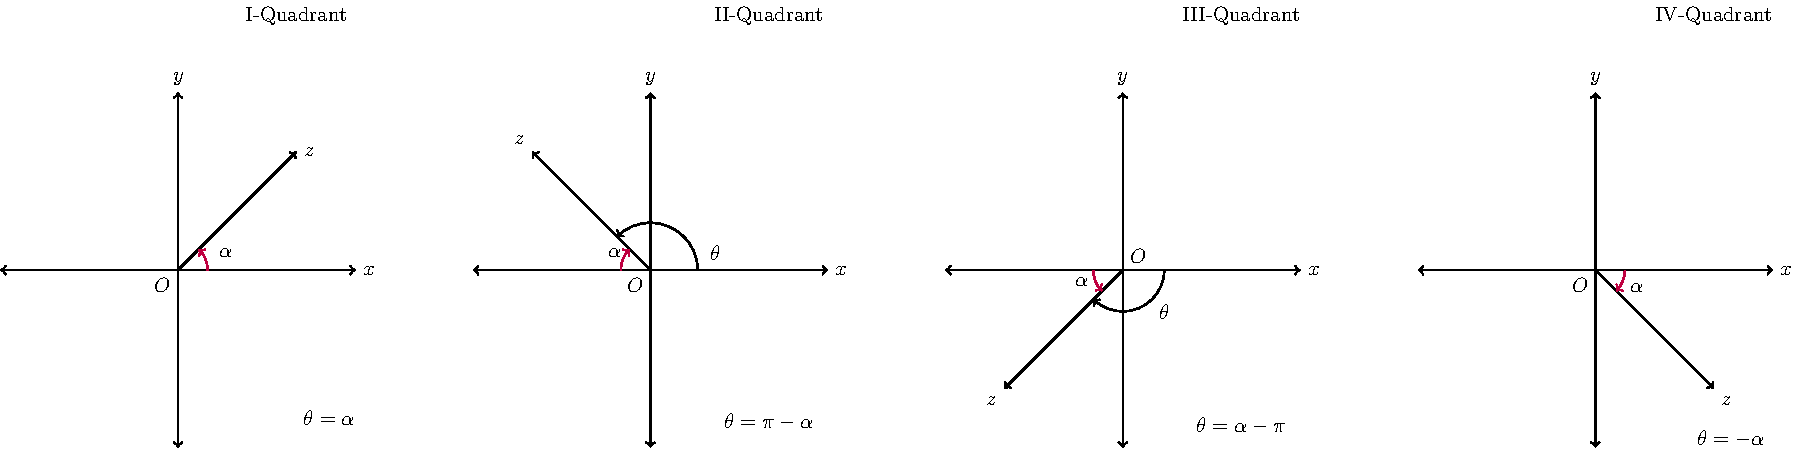
\includegraphics[scale=0.5]{FIG_MAT215/FIG4.pdf}
    \caption{Principle Argument of Complex Number}
    \label{fig4}
\end{figure}
\FloatBarrier
\noindent $(x, y) \rightarrow$ coordinate of the complex number in 2D complex plane.\par 
\noindent $(\pi, \theta) \rightarrow$ polar coordinate of the complex number in the complex plane. \par 
\noindent Where,
$$
r=\sqrt{x^2+y^2}=|x+i y|=\text { modulus or absolute value of } z=x+i y
$$
and $\theta=\operatorname{Arg}(z)$\par 
\noindent Then a complex number of the form $z=x+i y$ can be represented using polar coordinate as,
$$
\begin{aligned}
z=x+i y & =r \cos \theta+i r \sin \theta \\
& =r(\cos \theta+i \sin \theta)
\end{aligned}
$$
\begin{figure}[ht!]
    \centering
    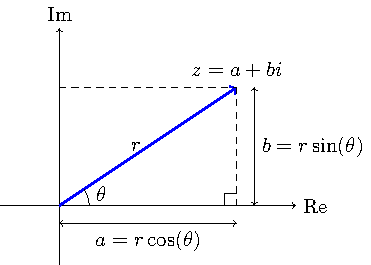
\includegraphics{FIG_MAT215/FIG5.pdf}
    \caption{}
    \label{fig5}
\end{figure}
\FloatBarrier
\begin{ex}
    Find the principal argument of the following complex numbers.\par 
(a) $1-i \quad $
(b) $2+2 \sqrt{3} i\quad$
(c) $4 \mathrm{i}\quad $\par 
\noindent \textbf{Solution:}\par 
\noindent (a) Principal argument, $\displaystyle \operatorname{Arg}(z)=-\tan ^{-1}\left(\left|\frac{y}{x}\right|\right)$
$$
\begin{aligned}
& =-\tan ^{-1}(1) \\
& =-\frac{\pi}{4}
\end{aligned}
$$
\noindent (b) Principal argument, $\displaystyle \operatorname{Arg}(z)=+\tan ^{-1}\left(\left|\frac{y}{x}\right|\right)$
$$
\begin{aligned}
& =\tan ^{-1}\left(\frac{2 \sqrt{3}}{2}\right) \\
& =\tan ^{-1}(\sqrt{3})=\frac{\pi}{3}
\end{aligned}
$$
\noindent (c) Principal argument, $\displaystyle \operatorname{Arg}(z)=\tan ^{-1}\left(\frac{4}{0}\right)=\frac{\pi}{2}$
\end{ex}
\begin{ex}
  Consider two complex number  $z_1=-i \quad, \quad z_2=-i+4$\par 
\noindent (i) Plot $z_1$ and $z_2$\par 
\noindent (ii) Find the modulus and principal argument of $z_1$ and $\displaystyle z_2$ $$ \quad \left[\textbf{Answer: }  r_1=1, \theta_1=-\pi / 2; \quad r_2=\sqrt{17},  \theta_2=\pi-\tan ^{-1}\left(\frac{1}{4}\right)\right]$$
\noindent (iii) Show that, $\left|z_1\right|=\left|\bar{z}_1\right|$, where $\bar{z}_1$ is the complex conjugate of $z_1$.\par 
\noindent (iv) Find, $z_1 z_2$ and $\cfrac{z_1}{z_2}$
\end{ex}
\begin{ex}
Convert $\displaystyle z=4 e^{-i \cfrac{\pi}{3}}$ in Cartesian coordinate system.\par 
\noindent \textbf{Solution:} Here, $\pi=4, \quad \theta=-\frac{\pi}{3}$
$$
\begin{aligned}
& x=r \cos \theta=4 \cos \left(-\frac{\pi}{3}\right)=4 \frac{1}{2}=2 \\
& y=r \sin \theta=4 \sin \left(-\frac{\pi}{3}\right)=-4 \frac{\sqrt{3}}{2}=-2 \sqrt{3}
\end{aligned}
$$

\noindent So, in Cartesian form, $z=2-2 \sqrt{3} i$. 
\end{ex}
\begin{ex}
    Convert $z=\sqrt{3}+2 \sqrt{3}i$  in the polar form.
\end{ex}

\section{De Moiver's Theorem}
Let $z_1=x_1+i y_1=r_1\left(\cos \theta_1+i \sin \theta_1\right)$ and $z_2=x_2+i y_2=r_2\left(\cos \theta_2+i \sin \theta_2\right)$, then we can show that
\begin{align}
z_1 z_2 & =r_1 r_2\left\{\cos \left(\theta_1+\theta_2\right)+i \sin \left(\theta_1+\theta_2\right)\right\} \\
\frac{z_1}{z_2} & =\frac{r_1}{r_2}\left\{\cos \left(\theta_1-\theta_2\right)+i \sin \left(\theta_1-\theta_2\right)\right\}
\end{align}
A generalization of (1.1) leads to
$$
z_1 z_2 \cdots z_n=r_1 r_2 \cdots r_n\left\{\cos \left(\theta_1+\theta_2+\cdots+\theta_n\right)+i \sin \left(\theta_1+\theta_2+\cdots+\theta_n\right)\right\}
$$
and if $z_1=z_2=\cdots=z_n=z$ this becomes
$$
z^n=\{r(\cos \theta+i \sin \theta)\}^n=r^n(\cos n \theta+i \sin n \theta)
$$
which is often called De Moivre's theorem.
\section{nth-Root of Complex Numbers}
Any nonzero complex number has exactly $n\in N$ distinct $n$-th roots. The roots lie on a circle of radius $|z|$ centered at the origin and spaced out equally by angles of $\displaystyle\frac{2\pi}{n}$. 
\begin{defn}
    A number $w$ is called $n$-th root of the complex number $z$ if $\displaystyle \omega^n=z$ and we can write $\displaystyle \omega=z^{\frac{1}{n}}$. 
\end{defn}
\begin{ex}
Find the $n$-th root of the complex number of the form $z=\pi e^{i \theta}$

\noindent \textbf{Solution:} Let $z_0=r_0 e^{i \theta_0}$ be the $n$-th root of $z$.
So,
$$
\begin{aligned}
& z_0^n=z \\
\Rightarrow & z_0^n=r e^{i \theta} \\
\Rightarrow & \left(r_0 e^{i \theta_0}\right)^n=r e^{i \theta} \\
\Rightarrow & r_0^n e^{i n \theta_0}=r e^{i \theta}
\end{aligned}
$$
which implies that, $\displaystyle r_0^n=r \Rightarrow r_0=r^{\frac{1}{n}}$ \par \noindent and $\displaystyle n \theta_0=\theta+2 k \pi \quad\{$ where $k=0, \pm 1, \pm 2, \ldots\}$

\noindent Now,
\begin{align*}
   \text{for } & k=0, \quad n \theta_0=\theta \Rightarrow \theta_0=\frac{\theta}{n}\\
   \text{for } & k=1, \quad n \theta_0=\theta+2 \pi \Rightarrow \theta_0=\frac{\theta}{n}+\frac{2 \pi}{n}\\
   \text{for } & k=2, \quad n \theta_0=\theta+4 \pi \Rightarrow \theta_0=\frac{\theta}{n}+\frac{4 \pi}{n}\\
   \text{for } & k=n-1, \quad n \theta_0=\theta+2 \pi(n-1) \Rightarrow \theta_0=\frac{\theta}{n}+\frac{2 \pi(n-1)}{n}\\
   \text{for } & k=n, \quad n \theta_0=\theta+2 n \pi \Rightarrow \theta_0=\frac{\theta}{n}+2 \pi \text{\hspace{3.5cm} (already found)}\\
   \text{for } & k=n+1, \quad n \theta_0=\theta+2 \pi(n+1) \Rightarrow \theta_0=\frac{\theta}{n}+\frac{2\pi}{n}+2 \pi \text{\hspace{0.9cm} (already found)}\\
   \vdots\\
   \text{for } & k=-1, \quad n \theta_0=\theta-2 \pi \Rightarrow \theta_0=\frac{\theta}{n}+\frac{2\pi(n-1)}{n}\text{\hspace{2.2cm} (already found)}\\
   \vdots\\
   \text{and }& \text{so on}
\end{align*}
As we are getting same root repeatedly, distinct $n$-roots are,
$$
\left.\begin{array}{l}
k=0 \longrightarrow z_1=r^{1/n}exp\left(i\frac{\theta}{n}\right) \\
k=1 \longrightarrow z_2=r^{1/n}exp\left(i\frac{2 \pi+\theta}{n}\right) \\
k=2 \longrightarrow z_3=r^{1/n}exp\left(i\frac{4 \pi+\theta}{n}\right) \\
\vdots \\
k=(n-2) \longrightarrow z_{n-1}=r^{1/n}exp\left(i\frac{2 \pi(n-2)+\theta}{n}\right) \\
k=(n-1) \longrightarrow z_{n}=r^{1/n}exp\left(i\frac{2 \pi(n-1)+\theta}{n}\right)
\end{array}\right\} 
$$
\end{ex}
\begin{ex}

\noindent (i) Find all values of $z$ such that $z^5=-32$. (ii) Locate these values in the complex plane.\par 

\noindent \textbf{Solution:} \par 
\noindent (i) The polar form of the given complex number, $\displaystyle z=-32=32e^{i\pi}$\par 
\noindent So, \begin{align*}
    &z_0^5=-32\hspace{3cm}\\
    \Rightarrow & (r_0e^{i\theta_0})^5=32e^{i\pi}\\
    \Rightarrow & r_0^5e^{i5\theta_0}=32e^{i\pi}
\end{align*}
Thus, $r_0=2$ \par 
\noindent and $5\theta_0=\pi+2\pi k$, where $k=0,1,2,3,4$\par 
\noindent Thus we will get the 5th root as follows, 
$$r_0e^{\frac{\pi+2\pi k}{5}} \quad \quad \text{where }k=0,1,2,3,4$$
More specifically, 
$$2exp\left(i\frac{\pi}{5}\right),\quad 2exp\left(i\frac{3\pi}{5}\right),\quad 2exp\left(i\frac{5\pi}{5}\right),\quad 2exp\left(i\frac{7\pi}{5}\right),\quad \text{and}\quad 2exp\left(i\frac{9\pi}{5}\right)$$
\end{ex}
\noindent (ii) Thus, the graphical representation of the roots are, \\
\begin{figure}[!ht]
    \centering
    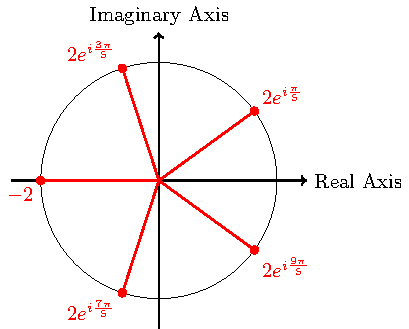
\includegraphics{FIG_MAT215/FIG6.pdf}
    \caption{Graphical representation of 5 roots}
    \label{fig6}
\end{figure}
\FloatBarrier
\begin{ex}
    Find the 4-th root of $-2\sqrt{3}-2i$ and locate them graphically. \par 
    \noindent \textbf{Solution:} \par 
    \noindent The polar form of the given complex number, $\displaystyle z=-2\sqrt{3}-2i=4e^{-i2\pi/3}$\par 
\noindent So, \begin{align*}
    &z_0^4=-2\sqrt{3}-2i\hspace{3cm}\\
    \Rightarrow & (r_0e^{i\theta_0})^4=4e^{-i2\pi/3}\\
    \Rightarrow & r_0^4e^{i4\theta_0}=4e^{-i2\pi/3}
\end{align*}
Thus, $r_0=\sqrt{2}$ \par 
\noindent and $4\theta_0=-2\pi/3+2\pi k$, where $k=0,1,2,3$\par 
\noindent Thus we will get the 4th root as follows, 
$$r_0e^{\frac{-2\pi/3+2\pi k}{4}} \quad \quad \text{where }k=0,1,2,3$$
More specifically, 
$$\sqrt{2}exp\left(-i\frac{\pi}{6}\right),\quad \sqrt{2}exp\left(i\frac{\pi}{3}\right),\quad \sqrt{2}exp\left(i\frac{5\pi}{6}\right),\quad  \text{and}\quad \sqrt{2}exp\left(i\frac{4\pi}{3}\right)$$
Graphically, 
\begin{figure}[!ht]
    \centering
    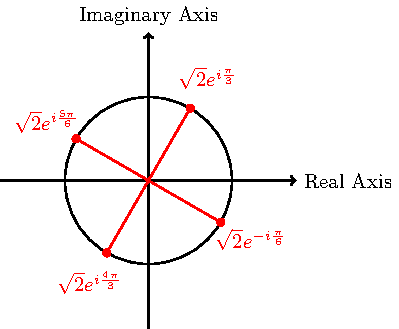
\includegraphics{FIG_MAT215/FIG7.pdf}
    \caption{Graphical representation of 4 roots}
    \label{fig7}
\end{figure}
\FloatBarrier
\end{ex}
\begin{ex}
    Find the 6-th root of $-1+\sqrt{3}i$ and locate them graphically. \par 
    \noindent \textbf{Solution:} \par 
    \noindent The polar form of the given complex number, $\displaystyle z=-1+\sqrt{3}i=2e^{i2\pi/3}$\par 
\noindent So, \begin{align*}
    &z_0^6=-1+\sqrt{3}i\hspace{3cm}\\
    \Rightarrow & (r_0e^{i\theta_0})^6=2e^{i2\pi/3}\\
    \Rightarrow & r_0^6e^{i6\theta_0}=2e^{i2\pi/3}
\end{align*}
Thus, $\displaystyle r_0=2^{(1/6)}$ \par 
\noindent and $6\theta_0=2\pi/3+2\pi k$, where $k=0,1,2,3,4,5$\par 
\noindent Thus we will get the 6th root as follows, 
$$r_0e^{\frac{2\pi/3+2\pi k}{6}} \quad \quad \text{where }k=0,1,2,3,4,5$$
More specifically, 
$$2^{(1/6)}exp\left(i\frac{\pi}{9}\right),\quad 2^{(1/6)}exp\left(i\frac{4\pi}{9}\right),\quad 2^{(1/6)}exp\left(i\frac{7\pi}{9}\right),$$
$$\quad 2^{(1/6)}exp\left(i\frac{10\pi}{9}\right), \quad 2^{(1/6)}exp\left(i\frac{13\pi}{9}\right), \quad  \text{and}\quad 2^{(1/6)}exp\left(i\frac{16\pi}{9}\right)$$
Graphically, 
\begin{figure}[!ht]
    \centering
    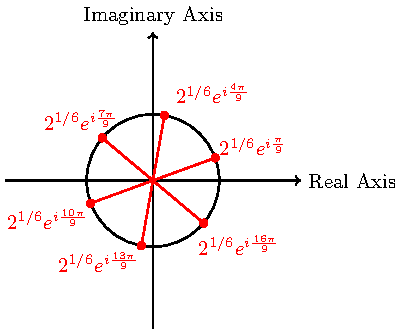
\includegraphics{FIG_MAT215/FIG8.pdf}
    \caption{Graphical representation of 4 roots}
    \label{fig7}
\end{figure}
\FloatBarrier
\end{ex}
\section{Graphical Representation of Complex Regions}
In this explainer, we will learn how to identify regions in the complex plane.
\begin{ex}
    Describe each of the region graphically, 
    $$(a) \quad \left|\frac{z-3}{z+3} \right|=2 \quad (b) \quad \left|\frac{z-3}{z+3} \right|<2$$
    \noindent \textbf{Solution:}\par 
    \noindent (a) \begin{align*}
        & \left|\frac{z-3}{z+3} \right|=2 \quad \\
        \Rightarrow & \mid z-3 \mid =2\mid z+3 \mid \\
        \Rightarrow & (x+5)^2+y^2=16 \quad [\text{After substituting } z=x+iy]
    \end{align*}
    Graphically, \begin{figure}[ht!]
        \centering
        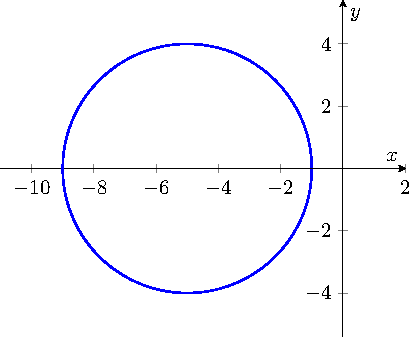
\includegraphics{FIG_MAT215/FIG9.pdf}
        \label{fig 9}
    \end{figure}
    \FloatBarrier
    (b) \begin{align*}
        &  \quad \left|\frac{z-3}{z+3} \right| < 2\\
        \Rightarrow & (x+5)^2+y^2>16
    \end{align*}
    Graphically, \begin{figure}[ht!]
        \centering
        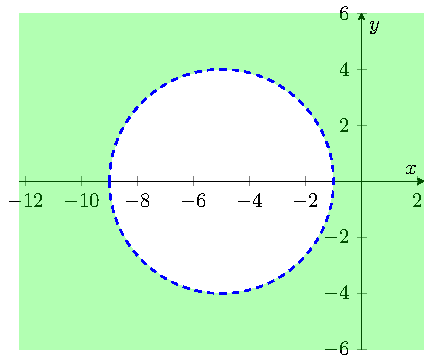
\includegraphics{FIG_MAT215/FIG10.pdf}
        \label{fig 10}
    \end{figure}
    \FloatBarrier
\end{ex}

\begin{ex}
    Describe each of the region graphically, 
    $$(a)\quad 1<\mid z+i \mid \leq 2 \quad (b)  \quad Re(z^2)>1 \quad (c) \quad Im(z^2)<4$$
    \noindent \textbf{Solution:} \par 
    \noindent (a) \begin{align*}
        & \quad 1<\mid z+i \mid \leq 2\\
        \Rightarrow & \quad 1<\mid x+iy+i \mid \leq 2\\
        \Rightarrow & 1<\sqrt{x^2+(1+y)^2} \leq 2 \\
        \Rightarrow & 1^2 < x^2+(1+y)^2 \leq 2^2
    \end{align*}
    Graphically, \begin{figure}[ht!]
        \centering
        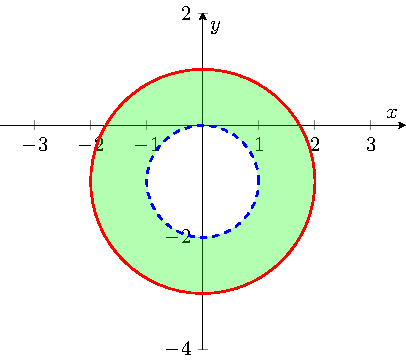
\includegraphics{FIG_MAT215/FIG11.pdf}
        \label{fig 11}
    \end{figure}
    \FloatBarrier
    \noindent (b) \begin{align*}
        & Re(z^2) > 1\\
        \Rightarrow & Re(x^2-y^2+i2xy)>1 \\
        \Rightarrow & x^2-y^2 >1
    \end{align*}
    Graphically, \begin{figure}[ht!]
        \centering
        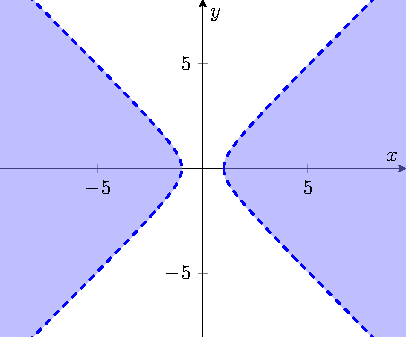
\includegraphics[scale=0.9]{FIG_MAT215/FIG12.pdf}
        \label{fig 12}
    \end{figure}
    \FloatBarrier
    \noindent (c) \begin{align*}
        & Im(z^2) < 4\\
        \Rightarrow & Im(x^2-y^2+i2xy)<4 \\
        \Rightarrow & xy <2
    \end{align*}
    Graphically, \begin{figure}[ht!]
        \centering
        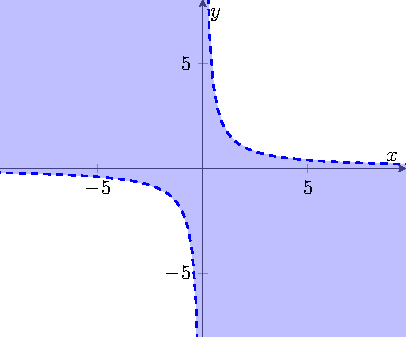
\includegraphics{FIG_MAT215/FIG13.pdf}
        \label{fig 13}
    \end{figure}
    \FloatBarrier
\end{ex}

\section{Exercise}
\begin{exercise}
    Express each of the following complex numbers in polar form, 
    $$(a)\quad  2+2\sqrt{3},\quad (b)\quad -5+5i, \quad \text{and }\quad  (iii)\quad -\sqrt{6}-\sqrt{2}i$$
\end{exercise}
\begin{exercise}
    Find the square root of $-15-8i$. 
\end{exercise}
\begin{exercise}
    Solve the equation $\displaystyle z^2+(2i-3)z+5-i=0$
\end{exercise}
\begin{exercise}
    Find all the 10-th root of unity. 
\end{exercise}
\begin{exercise}
    Find the indicated roots and locate them graphically, 
    $$(a) \quad (64)^{1/6}\quad (b) \quad (i)^{2/3} \quad (c)\quad (-1+i)^{1/3} \quad (d) \quad (-27i)^{1/6} \quad (e) \quad (-11-2i)^{1/3}$$
\end{exercise}
\begin{exercise}
    Describe each of the region graphically, 
    $$(i)\quad Re(z)>1 \quad (ii)\quad \mid 2z+3 \mid >4 \quad (iii) \quad 1< \mid z-2i \mid 2 \quad (iv) \quad \mid z+1-i \mid \leq \mid z-1+i \mid $$
    $$(v) \quad Re(1/z)>1 \quad (vi) \quad \mid z-4 \mid \geq \mid z \mid \quad (vii) \quad Re(1/z)\leq \frac{1}{2} \quad (viii) \quad \mid z-2 \mid \leq \mid z+2 \mid$$
\end{exercise}
\begin{exercise}
    Using the properties of Conjugate and modulus to show that, $$\mid 2z+3\bar{z}\mid \leq 4 \mid Re(z) \mid +\mid z\mid$$
\end{exercise}
\begin{exercise}
    Prove that, $\mid z+2i \mid + \mid z-2i \mid =6$  represents an ellipse.
\end{exercise}
\begin{exercise}
    Describe graphically the region represented by each of the following, 
    $$(i) \quad 1<\mid z+i \mid \leq 2 \quad (ii) \quad Re(z^2)>1 \quad (iii) \quad Im(z^2)=4 \quad (iv) \quad \mid z-3 \mid - \mid z+3 \mid =4$$
\end{exercise}
